% Subdocumento 9. Plan de calidad.

\begin{resumenApertura}
Este plan define cómo se verificará la calidad del servicio, el software y los componentes telemáticos de la solución para Transportes Curimón S.A. Establece criterios de aceptación trazables, niveles de prueba, controles de calidad y evidencia de conformidad. La disponibilidad de servicio se fija en 99,9\,\%; la continuidad local considera el mínimo de 72 horas exigido en RT-03.10. Los perfiles de carga se conciliarán con la arquitectura y las actividades de calidad se vincularán al plan de trabajo.
\begin{recibe}
  \item Criterios de calidad y aceptación vinculados a las bases y a la matriz de requerimientos.
  \item Estrategia de verificación desde pruebas unitarias hasta aceptación operacional.
  \item Registro de evidencias, defectos y decisiones para cada hito.
  \item Parámetros de carga y actividades de prueba vinculados con arquitectura, hardware y cronograma.
\end{recibe}
\end{resumenApertura}

\section{Plan de Calidad}\label{sec:9-plan-calidad}

El plan aplica controles preventivos y verificaciones basadas en riesgo a cada incremento de software, configuración de infraestructura y equipo embarcado. Los criterios de servicio provienen de las bases; los umbrales adicionales de ingeniería se identifican como propuestas y solo pasan a ser bloqueantes después de su aprobación técnica y contractual.


\subsection{Modelo de calidad y controles verificables}\label{sec:9-modelo}

Se utiliza el modelo de calidad de producto ISO/IEC 25010:2023, con nueve características \parencite{iso25010_2023}. No constituye una certificación de audIT ni demuestra conformidad por nombrarlo. Cada característica se transforma en una pregunta de ensayo y en evidencia conservada.

La adecuación funcional se verifica contrastando entradas, reglas de despacho, jornada, documentos y salidas contra un oráculo independiente; cualquier autorización ilegal es fallo, aunque otros casos aprueben. La eficiencia de desempeño se mide mediante percentiles y distribución por unidad: asignación p95 de hasta treinta segundos, DET hasta noventa segundos y sincronización hasta veinte minutos por camión tras setenta y dos horas sin cobertura. Una media favorable no compensa una unidad fuera del límite.

La compatibilidad se prueba con contratos versionados de ERP, GPS, TMS y dispositivos; duplicados, cambios de esquema y respuesta ausente no pueden producir doble emisión o pérdida de evidencia. La capacidad de interacción se verifica con tareas representativas de despacho, taller y conductor detenido; se registran finalización, errores y necesidad de asistencia, sin inventar una tasa de éxito ya medida.

La fiabilidad se verifica con disponibilidad real E2E de al menos 99,9\,\%, continuidad local y ejercicios de recuperación con RTO de hasta cuatro horas y RPO de hasta quince minutos. La seguridad se comprueba mediante autorización por titular, alcance y vigencia, revocación efectiva, aislamiento entre clientes y protección de evidencia; un acceso no autorizado bloquea la promoción.

La mantenibilidad se verifica con revisión, análisis estático, pruebas de regresión y cobertura automatizada de la lógica de negocio de al menos 70\,\%; 80\,\% es un objetivo adicional. La flexibilidad se comprueba en los modelos e interfaces homologados, con actualización/reversión y perfiles nominales y de estrés: no se presume compatibilidad con cualquier camión. La seguridad operacional se verifica mediante bloqueo ante jornada ausente, habilitación vencida o documento no conforme; la interacción del conductor se admite únicamente detenido. Dos autorizaciones comerciales no levantan esos bloqueos legales.



La madurez del desarrollo seguro se gestiona mediante evaluación inicial y reevaluación anual con OWASP SAMM o marco equivalente (\transv{RT-11.28}{24}, carácter deseable). El resultado identifica práctica, evidencia, brecha, responsable y acción; no se declara una madurez alcanzada ni una certificación CMMI. Como controles adicionales de ingeniería, audIT adopta complejidad ciclomática $v(G)\le15$ por función, duplicación menor que 3\,\% del código analizado y cero ciclos en el grafo de dependencias entre módulos de negocio. Se conservan versión del analizador, exclusiones justificadas, denominador y grafo. Una función que excede quince caminos independientes requiere refactorización o descomposición antes de promocionar; un ciclo o acceso directo a datos ajenos incumple el límite de contexto. Estos controles bloquean promoción como compromisos de audIT, sin atribuir los números a las bases. La revisión por pares verifica que reducir una métrica no oculte lógica o suprima pruebas.

El flujo incorpora SAST, composición, DAST y escaneo de imágenes con bloqueo de hallazgos críticos (\transv{RT-11.22}{24}); entrega SBOM por versión (RT-11.23) y firma/procedencia conforme a SLSA nivel 3 o superior (RT-11.24). El reporte relaciona artefacto, huella, pipeline y promoción autorizada; una firma aislada no demuestra cumplimiento de SLSA.

Estos controles relacionan calidad con consecuencias operacionales concretas: el análisis de seguridad no sustituye la comprobación de jornada, y la cobertura de código no acredita disponibilidad. T-13 organiza la ejecución y T-17 contiene los 120 casos diseñados y sus criterios, sin presentar resultados antes de ensayar.

\subsection{Objetivos y métricas de aceptación}\label{sec:9-metricas}

La \tabref{9-metricas-calidad} distingue los compromisos trazados de los objetivos internos que aún deben validarse. Los objetivos internos no sustituyen ni rebajan los umbrales contractuales.

\begin{tabla}[ancho=completo]{Métricas de calidad y trazabilidad}{9-metricas-calidad}{L{31mm} X L{37mm} L{43mm}}
Métrica & Criterio & Naturaleza y fuente & Evidencia \\ \midrule
Disponibilidad de servicios críticos & $\ge 99{,}9\%$ mensual E2E & Contractual: Art. 20 FEP01, p. 14; RT-10.01 FEP02, p. 22 & Medición real de transacciones E2E; monitoreo sintético complementario y reporte \\
Recuperación ante desastre & RTO $\le 4$ h; RPO $\le 15$ min & Contractual: RT-07.04 FEP02, p. 17 & Informe fechado de ejercicio de recuperación \\
Retención local sin conectividad & Al menos 72 h, sin pérdida ni corrupción & Contractual: RT-03.10, p. 31 & Registro de desconexión, almacenamiento y sincronización \\
Cobertura de pruebas unitarias & Mínimo $\ge70\%$; objetivo adicional $\ge80\%$ & RT-04.11 FEP02, p. 11; 80\% adicional & Reporte de cobertura por versión \\
Perfil de carga y latencia & Carga y concurrencia sustentadas en el dimensionamiento & Perfil de ensayo con hipótesis declaradas & Script versionado, parámetros aprobados y resultados \\
\end{tabla}

La disponibilidad se medirá sobre el servicio punta a punta y con la ventana, exclusiones y método de cómputo que establezcan las bases. El requisito de retención local es 72 h; la capacidad ampliada de 288 h es una propuesta de arquitectura física y su verificación depende del diseño y perfil de muestreo que se confirmen.

\subsection{Responsabilidades de calidad}\label{sec:9-responsabilidades}

La jefatura de aseguramiento administra el plan, la matriz de trazabilidad y el registro de defectos. Desarrollo corrige hallazgos y adjunta evidencia; QA prepara o revisa los casos y comunica resultados; arquitectura y hardware confirman los parámetros de sus componentes. La aceptación del mandante permanece en la contraparte técnica designada. La asignación de responsables y la segregación de funciones del flujo de integración se vinculan a las funciones y dedicaciones de S7/T-15.

\section{Estrategia de Aseguramiento de Calidad}\label{sec:9-estrategia}

La verificación combina inspección, análisis automatizado y pruebas dinámicas. Se ejecutará sobre versiones identificadas y ambientes controlados. Las herramientas, los umbrales de seguridad y las autorizaciones de despliegue se especificarán en el diseño del flujo de integración; no se declara que los controles descritos ya estén implantados ni que las pruebas se hayan ejecutado.


La \figref{9-proceso-calidad} muestra el recorrido general desde el criterio contractual hasta la aceptación. El detalle de niveles, datos y decisiones se desarrolla después de la figura.

\begin{figuraNativa}{Recorrido de calidad, evidencia y aceptación}{9-proceso-calidad}
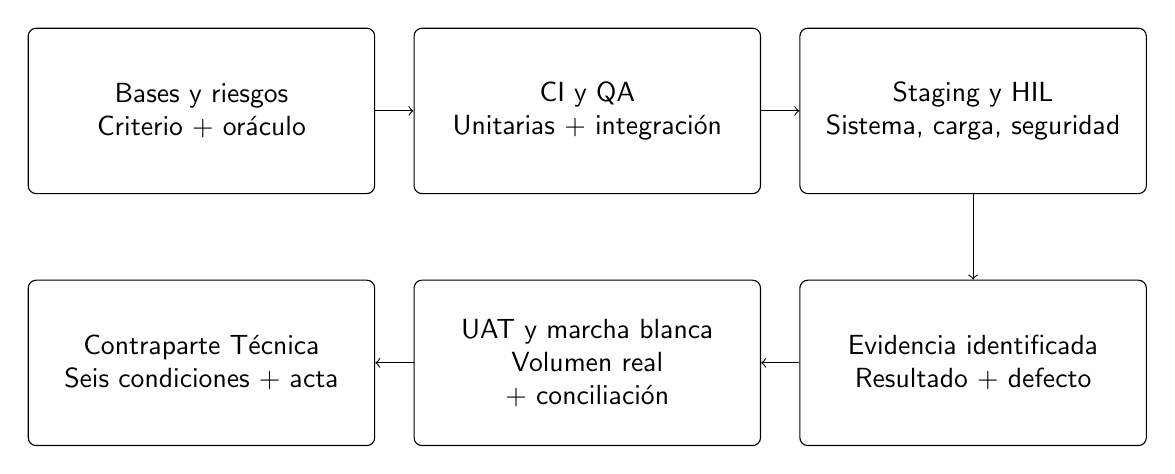
\begin{tikzpicture}[x=1mm,y=1mm,every node/.style={font=\fontsize{10}{12}\selectfont\sffamily,align=center},bloque/.style={draw,rounded corners=1mm,text width=40mm,minimum height=21mm,inner sep=2mm}]
\node[bloque] (r) at (0,0) {Bases y riesgos\\Criterio + oráculo};
\node[bloque] (u) at (49,0) {CI y QA\\Unitarias + integración};
\node[bloque] (h) at (98,0) {Staging y HIL\\Sistema, carga, seguridad};
\node[bloque] (e) at (98,-32) {Evidencia identificada\\Resultado + defecto};
\node[bloque] (a) at (49,-32) {UAT y marcha blanca\\Volumen real + conciliación};
\node[bloque] (c) at (0,-32) {Contraparte Técnica\\Seis condiciones + acta};
\draw[->] (r)--(u);\draw[->] (u)--(h);\draw[->] (h)--(e);\draw[->] (e)--(a);\draw[->] (a)--(c);
\end{tikzpicture}
\end{figuraNativa}

El primer bloque fija el criterio antes de ejecutar; CI y QA detectan fallos de lógica y contratos antes de utilizar dispositivos o datos operacionales. Staging y HIL reproducen carga, desconexión y fallas con controles de reversión. El resultado conserva ambiente, versión, entradas y medición: una captura sin esos datos no permite reevaluar el ensayo. UAT comprueba tareas con usuarios designados; marcha blanca añade volumen real y estabilidad sostenida. La Contraparte Técnica formaliza el cierre solo cuando concurren las seis condiciones contractuales. Cualquier fallo devuelve el incremento a corrección y reevaluación, sin convertir la figura en evidencia de ejecución.

\subsection{Niveles, ambientes y datos de prueba}\label{sec:9-ambientes}

La secuencia propuesta es: pruebas unitarias en integración continua; pruebas de integración en QA; pruebas de sistema, rendimiento y seguridad en staging; ensayos de hardware en banco HIL; y aceptación de usuario en los terminales que confirme el plan de trabajo. Producción y recuperación ante desastres se usan solo en ejercicios autorizados, con ventana, respaldo y reversión aprobados.

Los datos de prueba serán sintéticos o anonimizados. El uso de datos operacionales requiere autorización, minimización, control de acceso y retención acordada. Cada conjunto de datos y script conservará versión, origen, parámetros y responsable, sin exponer datos personales reales.

\subsection{Criterios de entrada, salida y gestión de defectos}\label{sec:9-criterios}

Antes de iniciar una prueba deben estar identificados el requisito y el caso de prueba; disponible la versión y el ambiente; aprobados los datos, parámetros, umbrales y responsables; y definidos los respaldos y la reversión cuando corresponda. La concurrencia y las ráfagas se fijan con el perfil de S4; las ventanas de ensayo son las de \verSeccionFolio{sec:9-calendario-pruebas}.

Una prueba se cierra cuando se conserva el resultado reproducible, la evidencia, la versión y la evaluación contra criterios previamente aprobados. No se acepta el cierre de marcha blanca con incidentes críticos o altos abiertos atribuibles a la solución. Los defectos restantes requieren responsable, severidad, plazo acordado y aceptación documentada de la contraparte. Las categorías y plazos definitivos deben concordar con el contrato y el protocolo aprobado.

\subsection{Puertas de calidad propuestas}\label{sec:9-puertas}

La \tabref{9-puertas-calidad} establece puntos de control propuestos. La plataforma CI, los escáneres, los roles autorizadores y los umbrales no contractuales deben concordar con el diseño del flujo de integración y con T-13.

\begin{tabla}[ancho=completo]{Puertas de calidad y evidencia de salida}{9-puertas-calidad}{L{22mm} X L{49mm} L{39mm}}
Puerta & Control propuesto & Condición de salida & Evidencia \\ \midrule
G1 — Código & Revisión por pares y análisis estático & Compilación correcta; defectos bloqueantes corregidos; cobertura reportada & Revisión y reporte CI \\
G2 — Dependencias & Análisis de dependencias y configuración & Hallazgos evaluados y tratamiento aprobado & SBOM y reporte de escaneo \\
G3 — Integración & Contratos e intercambio entre servicios & Casos de integración trazados aprobados & Resultados y logs de integración \\
G4 — Sistema & Rendimiento, resiliencia y seguridad & Umbrales acordados antes del ensayo y cumplidos & Reporte de ejecución y configuración \\
G5 — Aceptación & Pruebas funcionales con usuarios designados & Acta de aceptación o lista de observaciones acordada & Casos ejecutados, incidencias y acta \\
G6 — Recuperación & Restauración y continuidad & RTO/RPO exigidos demostrados en ejercicio autorizado & Bitácora, marcas de tiempo y reporte \\
\end{tabla}

Una puerta fallida detiene la promoción del incremento hasta que se documente la corrección o una excepción autorizada. La configuración concreta del pipeline GitLab, los servicios cloud y las herramientas mencionadas en los borradores se conciliarán con la arquitectura lógica.

\section{Alineación con Plan de Trabajo}\label{sec:9-plan-trabajo}

Las pruebas deben preceder a los hitos de integración, despliegue y aceptación a los que dan evidencia. La secuencia siguiente organiza las evidencias que deben incorporarse a los paquetes de trabajo y al calendario de los Formularios T-14, T-15 y T-18.

\subsection{Secuencia de hitos de calidad}\label{sec:9-hitos}

La \tabref{9-hitos-calidad} relaciona cada hito con su actividad de aseguramiento, la evidencia de salida y la dependencia que permite ejecutarla.

\begin{tabla}[ancho=completo]{Secuencia de aseguramiento y dependencias de cronograma}{9-hitos-calidad}{L{30mm} X L{46mm} L{39mm}}
Hito & Actividad de calidad & Evidencia de salida & Dependencia \\ \midrule
Diseño y construcción & Revisar requisitos, riesgos, arquitectura de prueba y datos & Matriz de trazabilidad y casos revisados & T-12 y definición de diseño \\
Integración & Ejecutar pruebas unitarias, contratos e integración & Reportes identificados por versión & Diseño del flujo de integración \\
Validación de sistema & Ejecutar seguridad, carga, resiliencia y recuperación en staging/HIL & Informes reproducibles y defectos asociados & Dimensionamiento y ambientes disponibles \\
Aceptación de hito & Ejecutar protocolo, recopilar observaciones y emitir acta & Evidencias y pronunciamiento de contraparte & Cronograma contractual y plan de trabajo \\
Marcha blanca y cierre & Medir disponibilidad, incidencias y transferencia a soporte & Reporte del período y acta de conformidad & Ventana y criterios contractuales confirmados \\
\end{tabla}

Esta secuencia organiza las evidencias de calidad alrededor de los hitos, pero se aplica a las ventanas contractuales detalladas a continuación, sin declarar pruebas ejecutadas.


\subsection{Actividades de calidad ubicadas en el calendario}\label{sec:9-calendario-pruebas}

El calendario contractual establece las ventanas; la red vigente de S7/T-15 identifica las actividades A09 a A25 utilizadas aquí. Los códigos A son actividades verificables del cronograma, sin atribuirles la condición de diccionario completo de la EDT. La \tabref{9-ventanas-prueba} sintetiza dónde se produce la evidencia de cada transición.

\begin{tabla}[ancho=completo]{Ventanas de ensayo y actividad de cronograma}{9-ventanas-prueba}{L{29mm} L{28mm} L{43mm} X}
Ventana & Actividad S7 & Ensayos & Salida verificable \\ \midrule
Construcción E1 & A09/A10/A11 & Unitarias, integración y piloto HIL & Versión y regresión trazadas \\
M12, hito H5 & A12 & Carga, resiliencia, DR, seguridad y UAT E1 & Informe y defectos de certificación \\
M13--M15 & A15 & Marcha blanca E1 & Cuatro semanas y seis condiciones \\
M16, hito H7 & A19 & Producción E1 & Acta de su alcance \\
Construcción E2 & A20 & Regresión E1 y ensayos del incremento & Evidencia sin degradación E1 \\
M18, hito H10 & A22 & Carga, resiliencia, DR, seguridad y UAT E2 & Informe y defectos de certificación \\
M19--M20 & A24 & Marcha blanca E2 & Cuatro semanas y seis condiciones \\
M21, hito H12 & A25 & Producto final & Acta e inicio de operación \\
\end{tabla}

Las pruebas de carga utilizan el perfil aprobado de S4, conservando mezcla y concurrencia; resiliencia incluye desconexión embarcada de 72 h, terminal de 24 h y reconexión masiva. Cada ejercicio DR mide desde la declaración del incidente hasta servicio recuperado y contrasta el último dato recuperable con RPO; seguridad ofensiva se ejecuta con autorización, límites, datos de ensayo y reversión. Las cuatro familias producen informes independientes en A12/M12 y A22/M18, para evitar que un éxito funcional sustituya una comprobación no funcional. Antes de cada paso a producción y semestralmente en operación se ensayan resiliencia y DR; las pruebas de intrusión se ejecutan antes de cada paso a producción y anualmente, por tercero independiente de audIT, con informe íntegro y remediación (\transv{20.1}{34--35}; \transv{RT-11.20}{24}). La carga prueba los umbrales a 1,5 veces el peak declarado. La migración definitiva requiere dos ensayos previos con conciliación sin diferencias no explicadas. Estas comprobaciones complementan las certificaciones A12/A22 y conservan responsables, autorización y ventanas.

\subsection{Protocolo de aceptación, observaciones y acta}\label{sec:9-protocolo-aceptacion}

Para cada hito se identificará el entregable, la versión sometida, el criterio objetivo, el responsable de ejecución y la evidencia. La contraparte revisará el paquete dentro de los plazos previstos en las bases; las observaciones se registrarán con identificador, requisito relacionado, severidad, evidencia y respuesta. La versión corregida se reevalúa contra el mismo criterio y se conserva la trazabilidad de ambas revisiones.

Solo el acta de aceptación suscrita acredita el hito; el registro de observaciones no sustituye la conformidad exigida. La disponibilidad contractual es al menos 99,9\,\%; RTO máximo 4 h y RPO máximo 15 min; la retención local mínima es 72 h. Para el resto de los criterios, el valor medido, el umbral aprobado y la fuente deben constar en el acta, sin completar resultados antes de ejecutar las pruebas.

\subsection{Registro de evidencia y control de cambios}\label{sec:9-evidencias}

Cada evidencia incluirá identificador de requisito/caso, fecha, versión, ambiente, datos de prueba, herramienta, resultado, defectos y responsable. Los reportes y actas se almacenarán en el repositorio controlado del proyecto con permisos y retención definidos. Todo cambio de caso, parámetro o umbral conservará motivo, aprobador, impacto y versión afectada.

\subsection{Condiciones contractuales de calendario y aceptación}\label{sec:9-condiciones-contractuales}

\begingroup\emergencystretch=3em
El calendario de la \tabref{9-calendario-contractual} es obligatorio conforme al \art{17.1}{12--13}. M1 se cuenta desde el origen contractual efectivo; no se convierte la fecha de entrega de la oferta en inicio del contrato. Los puntos de control técnicos no sustituyen los hitos ponderados de E-25.\par\endgroup

\begin{tabla}[ancho=completo]{Calendario contractual y evidencia de transición}{9-calendario-contractual}{L{34mm} L{24mm} X}
Fase & Meses & Control y evidencia \\ \midrule
Desarrollo E1 & M1--M12 & Construcción, integración, migración, seguridad y certificación. \\
Marcha blanca E1 & M13--M15 & Tres meses supervisados; seis condiciones acumulativas de cierre. \\
Producción E1 & M16 & Sistema de registro oficial de su alcance. \\
Desarrollo E2 & M13--M18 & Solapamiento con E1; cierre del desarrollo en M18. \\
Marcha blanca E2 & M19--M20 & Dos meses supervisados; única fuente de verdad compartida. \\
Producción E2 & M21 & Aceptación final e inicio simultáneo de operación. \\
Operación & M21--M56 & Ambos alcances: 36 meses de soporte y servicio. \\
\end{tabla}

La convivencia exige frentes suficientes, integridad compartida y ausencia de degradación de E1 (\art{17.2}{13}); la nivelación se acredita mediante S7 y T-15. Ningún ensayo o congelamiento operacional desplaza estas fases.

Cada marcha blanca cierra solo cuando se cumplen simultáneamente las seis condiciones del \art{17.3}{13}: ningún incidente crítico ni alto abierto atribuible a la solución; volumen real comprometido durante al menos las cuatro últimas semanas; disponibilidad y respuesta cumplidas sostenidamente en ese mismo período; conciliación sin diferencias no explicadas; personal del cliente capacitado y certificado según plan aprobado; y acta suscrita por la Contraparte Técnica. Si no se cumplen, audIT extiende la marcha blanca a su costo, sin cargo adicional ni desplazamiento de fases siguientes y sujeto a las multas contractuales.

El cliente dispone de diez días hábiles para revisar y pronunciarse y audIT de diez días hábiles para subsanar. La segunda presentación con observaciones de igual naturaleza constituye atraso imputable a audIT (\art{18.3}{13}). La aceptación requiere acta suscrita; no procede aprobación por silencio. Cada ingreso adjunta artefacto, evidencia objetiva, trazabilidad y observaciones previas resueltas (\art{18.1 y 18.2}{13}). No se premarcan resultados, adjuntos, incidencias ni pronunciamientos. La aceptación no convalida defectos posteriores (\art{18.4}{13}).

\subsection{Controles mínimos trazados y método de medición}\label{sec:9-minimos-trazados}

La \tabref{9-minimos-trazados} concreta los criterios que deben incorporarse al catálogo de pruebas y sus reportes. Los parámetros adicionales no rebajan estos mínimos.

\begin{tabla}[ancho=completo]{Criterios contractuales de servicio y continuidad}{9-minimos-trazados}{L{31mm} L{36mm} X}
Control & Umbral & Fuente y evidencia \\ \midrule
Disponibilidad crítica E2E & $\ge99{,}9\%$ mensual & \art{20}{14}, \transv{RT-10.01}{22}: intentos, éxito/fallo y duración de transacciones reales correlacionadas. Monitoreo sintético complementario. \\
Red, cómputo, datos y portal & $\ge99{,}95\%$ por componente & FEP02, Cap. 7, pp. 17--18; sala Cap. 6: métricas por componente y conciliación con incidencias de negocio. \\
Recuperación & RTO $\le4$ h; RPO $\le15$ min & \transv{RT-07.04}{17}: conmutación real autorizada, tiempos y datos recuperados. \\
Asignación bloqueante & p95 $\le30$ s & \caso{RT-09.01}{32}; FEP02 Cap. 9: jornada previa, habilitaciones y equipo bajo carga declarada. \\
Documento de transporte & $\le90$ s & \caso{RT-09.01}{32}: documento conforme antes de mover carga; ERP contable como emisor tributario. \\
Emergencia y posición & $\le15$ s con cobertura; $\le2$ min & \caso{RT-09.01}{32}: tiempos origen/destino; publicación al cliente y cobertura documentada. \\
Costeo & $\le24$ h tras cierre & \caso{RT-05.29}{32}: consolidación con identificación de componentes aún no disponibles. \\
Cobertura de negocio & $\ge70\%$; objetivo adicional 80\% & \transv{RT-04.11}{11}: umbral bloqueante sobre lógica de negocio. No demuestra por sí solo corrección funcional. \\
Autonomía embarcada & $\ge72$ h sin cobertura & \caso{RT-03.10}{31}: posición, conducción, jornada, tiempos y documentos sin pérdida. 288 h es propuesta adicional. \\
Autonomía terminal & $\ge24$ h sin enlace exterior & \art{16.4}{12}; \transv{RT-03.10}{9}: mínimo transversal ante las 12 h del caso; operación degradada y conciliación. \\
Reconexión masiva & $\le20$ min por camión tras 72 h & \caso{RT-03.13}{31}: perfil explícito de 300 unidades simultáneas; medir por unidad, sin pérdida de jornada o esperas. \\
\end{tabla}

Los mínimos de infraestructura no acreditan éxito de la transacción: se mide la experiencia real de la persona usuaria, conforme a FEP02, Cap. 9. Los SLA del T-6 corresponden a experiencia histórica y no se alteran. El perfil de 300 unidades responde al escenario de varios cientos del Caso, numeral 14.2; la tasa de generación, tamaño y ráfaga se justifican en la memoria de cálculo.

En marcha la captura es automática y no se admite interacción manual. Solo se habilita interacción con el vehículo detenido. El titular controla autorización, alcance, vigencia y revocación de datos; la jornada previa de un conductor externo requiere evidencia autorizada y su ausencia no equivale a jornada cero ni habilita despacho. Llegada y salida se registran automáticamente sin instalar equipos en recintos de clientes (\caso{RT-09.01}{32}).

El cliente adquiere el hardware; audIT especifica cantidades, características, interoperabilidad, seguridad y reposición (Caso, Cap. 11; FEP02, Cap. 8). La sala de San Bernardo debe remediarse o reemplazarse y EXC-04 no excluye sus adecuaciones necesarias (\caso{RT-06.01}{32}). No se presupone equipamiento, API del ERP ni acceso autorizado a interfaces de fábrica.
